\documentclass[twoside]{book}

% Packages required by doxygen
\usepackage{fixltx2e}
\usepackage{calc}
\usepackage{doxygen}
\usepackage[export]{adjustbox} % also loads graphicx
\usepackage{graphicx}
\usepackage[utf8]{inputenc}
\usepackage{makeidx}
\usepackage{multicol}
\usepackage{multirow}
\PassOptionsToPackage{warn}{textcomp}
\usepackage{textcomp}
\usepackage[nointegrals]{wasysym}
\usepackage[table]{xcolor}

% Font selection
\usepackage[T1]{fontenc}
\usepackage[scaled=.90]{helvet}
\usepackage{courier}
\usepackage{amssymb}
\usepackage{sectsty}
\renewcommand{\familydefault}{\sfdefault}
\allsectionsfont{%
  \fontseries{bc}\selectfont%
  \color{darkgray}%
}
\renewcommand{\DoxyLabelFont}{%
  \fontseries{bc}\selectfont%
  \color{darkgray}%
}
\newcommand{\+}{\discretionary{\mbox{\scriptsize$\hookleftarrow$}}{}{}}

% Page & text layout
\usepackage{geometry}
\geometry{%
  a4paper,%
  top=2.5cm,%
  bottom=2.5cm,%
  left=2.5cm,%
  right=2.5cm%
}
\tolerance=750
\hfuzz=15pt
\hbadness=750
\setlength{\emergencystretch}{15pt}
\setlength{\parindent}{0cm}
\setlength{\parskip}{3ex plus 2ex minus 2ex}
\makeatletter
\renewcommand{\paragraph}{%
  \@startsection{paragraph}{4}{0ex}{-1.0ex}{1.0ex}{%
    \normalfont\normalsize\bfseries\SS@parafont%
  }%
}
\renewcommand{\subparagraph}{%
  \@startsection{subparagraph}{5}{0ex}{-1.0ex}{1.0ex}{%
    \normalfont\normalsize\bfseries\SS@subparafont%
  }%
}
\makeatother

% Headers & footers
\usepackage{fancyhdr}
\pagestyle{fancyplain}
\fancyhead[LE]{\fancyplain{}{\bfseries\thepage}}
\fancyhead[CE]{\fancyplain{}{}}
\fancyhead[RE]{\fancyplain{}{\bfseries\leftmark}}
\fancyhead[LO]{\fancyplain{}{\bfseries\rightmark}}
\fancyhead[CO]{\fancyplain{}{}}
\fancyhead[RO]{\fancyplain{}{\bfseries\thepage}}
\fancyfoot[LE]{\fancyplain{}{}}
\fancyfoot[CE]{\fancyplain{}{}}
\fancyfoot[RE]{\fancyplain{}{\bfseries\scriptsize Generated by Doxygen }}
\fancyfoot[LO]{\fancyplain{}{\bfseries\scriptsize Generated by Doxygen }}
\fancyfoot[CO]{\fancyplain{}{}}
\fancyfoot[RO]{\fancyplain{}{}}
\renewcommand{\footrulewidth}{0.4pt}
\renewcommand{\chaptermark}[1]{%
  \markboth{#1}{}%
}
\renewcommand{\sectionmark}[1]{%
  \markright{\thesection\ #1}%
}

% Indices & bibliography
\usepackage{natbib}
\usepackage[titles]{tocloft}
\setcounter{tocdepth}{3}
\setcounter{secnumdepth}{5}
\makeindex

% Hyperlinks (required, but should be loaded last)
\usepackage{ifpdf}
\ifpdf
  \usepackage[pdftex,pagebackref=true]{hyperref}
\else
  \usepackage[ps2pdf,pagebackref=true]{hyperref}
\fi
\hypersetup{%
  colorlinks=true,%
  linkcolor=blue,%
  citecolor=blue,%
  unicode%
}

% Custom commands
\newcommand{\clearemptydoublepage}{%
  \newpage{\pagestyle{empty}\cleardoublepage}%
}

\usepackage{caption}
\captionsetup{labelsep=space,justification=centering,font={bf},singlelinecheck=off,skip=4pt,position=top}

%===== C O N T E N T S =====

\begin{document}

% Titlepage & ToC
\hypersetup{pageanchor=false,
             bookmarksnumbered=true,
             pdfencoding=unicode
            }
\pagenumbering{roman}
\begin{titlepage}
\vspace*{7cm}
\begin{center}%
{\Large Battleship }\\
\vspace*{1cm}
{\large Generated by Doxygen 1.8.11}\\
\end{center}
\end{titlepage}
\clearemptydoublepage
\tableofcontents
\clearemptydoublepage
\pagenumbering{arabic}
\hypersetup{pageanchor=true}

%--- Begin generated contents ---
\chapter{Hierarchical Index}
\section{Class Hierarchy}
This inheritance list is sorted roughly, but not completely, alphabetically\+:\begin{DoxyCompactList}
\item \contentsline{section}{Game}{\pageref{classGame}}{}
\item \contentsline{section}{Main}{\pageref{classMain}}{}
\item \contentsline{section}{Player}{\pageref{classPlayer}}{}
\begin{DoxyCompactList}
\item \contentsline{section}{Bot}{\pageref{classBot}}{}
\item \contentsline{section}{User}{\pageref{classUser}}{}
\end{DoxyCompactList}
\item \contentsline{section}{Ship}{\pageref{classShip}}{}
\item \contentsline{section}{Test\+Game}{\pageref{classTestGame}}{}
\end{DoxyCompactList}

\chapter{Class Index}
\section{Class List}
Here are the classes, structs, unions and interfaces with brief descriptions\+:\begin{DoxyCompactList}
\item\contentsline{section}{\hyperlink{classBot}{Bot} \\*\hyperlink{classBot}{Bot} class }{\pageref{classBot}}{}
\item\contentsline{section}{\hyperlink{classGame}{Game} \\*Engine of a game }{\pageref{classGame}}{}
\item\contentsline{section}{\hyperlink{classGridPanel}{Grid\+Panel} \\*Panel representing board }{\pageref{classGridPanel}}{}
\item\contentsline{section}{\hyperlink{classGUIListener}{G\+U\+I\+Listener} \\*Listener class }{\pageref{classGUIListener}}{}
\item\contentsline{section}{\hyperlink{classMain}{Main} \\*\hyperlink{classMain}{Main} class to run a game }{\pageref{classMain}}{}
\item\contentsline{section}{\hyperlink{classMainGUI}{Main\+G\+UI} \\*\hyperlink{classMain}{Main} class }{\pageref{classMainGUI}}{}
\item\contentsline{section}{\hyperlink{classMainMenuPanel}{Main\+Menu\+Panel} \\*Panel of main menu }{\pageref{classMainMenuPanel}}{}
\item\contentsline{section}{\hyperlink{classPlayer}{Player} \\*\hyperlink{classPlayer}{Player} abstract class }{\pageref{classPlayer}}{}
\item\contentsline{section}{\hyperlink{classShip}{Ship} \\*\hyperlink{classShip}{Ship} class }{\pageref{classShip}}{}
\item\contentsline{section}{\hyperlink{classTestGame}{Test\+Game} \\*A J\+Unit test class to test \hyperlink{classGame}{Game} class }{\pageref{classTestGame}}{}
\item\contentsline{section}{\hyperlink{classUser}{User} \\*\hyperlink{classUser}{User} class }{\pageref{classUser}}{}
\end{DoxyCompactList}

\chapter{Class Documentation}
\hypertarget{classBot}{}\section{Bot Class Reference}
\label{classBot}\index{Bot@{Bot}}


\hyperlink{classBot}{Bot} class.  




Inheritance diagram for Bot\+:
\nopagebreak
\begin{figure}[H]
\begin{center}
\leavevmode
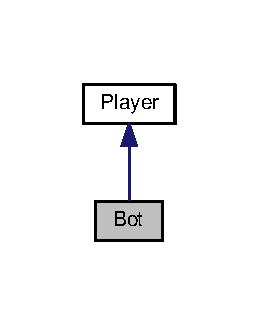
\includegraphics[width=124pt]{classBot__inherit__graph}
\end{center}
\end{figure}


Collaboration diagram for Bot\+:
\nopagebreak
\begin{figure}[H]
\begin{center}
\leavevmode
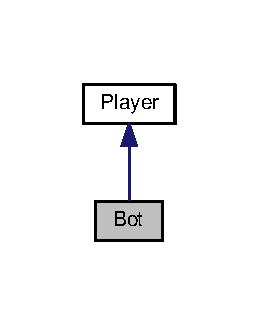
\includegraphics[width=124pt]{classBot__coll__graph}
\end{center}
\end{figure}
\subsection*{Public Member Functions}
\begin{DoxyCompactItemize}
\item 
\hyperlink{classBot_a3e856f881d832774e0a607435ca3793e}{Bot} (\hyperlink{classGame}{Game} game, int id)
\begin{DoxyCompactList}\small\item\em Constructor. \end{DoxyCompactList}\item 
void \hyperlink{classBot_a1f860395e5334c64f8cb50edb6cbca1f}{build\+Ships} ()
\begin{DoxyCompactList}\small\item\em Build ships. \end{DoxyCompactList}\item 
void \hyperlink{classBot_a259001d8480a450678ee85d570a9f206}{attack} ()\hypertarget{classBot_a259001d8480a450678ee85d570a9f206}{}\label{classBot_a259001d8480a450678ee85d570a9f206}

\begin{DoxyCompactList}\small\item\em Attack the opponent\textquotesingle{}s \hyperlink{classShip}{Ship}\textquotesingle{}s. \end{DoxyCompactList}\end{DoxyCompactItemize}
\subsection*{Additional Inherited Members}


\subsection{Detailed Description}
\hyperlink{classBot}{Bot} class. 

Class representing a simple AI to play against. 

\subsection{Constructor \& Destructor Documentation}
\index{Bot@{Bot}!Bot@{Bot}}
\index{Bot@{Bot}!Bot@{Bot}}
\subsubsection[{\texorpdfstring{Bot(\+Game game, int id)}{Bot(Game game, int id)}}]{\setlength{\rightskip}{0pt plus 5cm}Bot.\+Bot (
\begin{DoxyParamCaption}
\item[{{\bf Game}}]{game, }
\item[{int}]{id}
\end{DoxyParamCaption}
)\hspace{0.3cm}{\ttfamily [inline]}}\hypertarget{classBot_a3e856f881d832774e0a607435ca3793e}{}\label{classBot_a3e856f881d832774e0a607435ca3793e}


Constructor. 


\begin{DoxyParams}{Parameters}
{\em game} & \hyperlink{classGame}{Game} object. \\
\hline
{\em id} & id of a player. \\
\hline
\end{DoxyParams}


\subsection{Member Function Documentation}
\index{Bot@{Bot}!build\+Ships@{build\+Ships}}
\index{build\+Ships@{build\+Ships}!Bot@{Bot}}
\subsubsection[{\texorpdfstring{build\+Ships()}{buildShips()}}]{\setlength{\rightskip}{0pt plus 5cm}void Bot.\+build\+Ships (
\begin{DoxyParamCaption}
{}
\end{DoxyParamCaption}
)\hspace{0.3cm}{\ttfamily [inline]}}\hypertarget{classBot_a1f860395e5334c64f8cb50edb6cbca1f}{}\label{classBot_a1f860395e5334c64f8cb50edb6cbca1f}


Build ships. 

A method to build ships. 

The documentation for this class was generated from the following file\+:\begin{DoxyCompactItemize}
\item 
src/Bot.\+java\end{DoxyCompactItemize}

\hypertarget{classGame}{}\section{Game Class Reference}
\label{classGame}\index{Game@{Game}}
\subsection*{Public Member Functions}
\begin{DoxyCompactItemize}
\item 
{\bfseries Game} (int game\+Type, int user\+Interface)  throws I\+O\+Exception \hypertarget{classGame_ae0ca81a868814b02a8267768494527b2}{}\label{classGame_ae0ca81a868814b02a8267768494527b2}

\item 
{\bfseries Game} (int user\+Interface, boolean is\+Server)  throws I\+O\+Exception \hypertarget{classGame_af7ee3d5189c58ed74d0cb7783ce64632}{}\label{classGame_af7ee3d5189c58ed74d0cb7783ce64632}

\item 
\hyperlink{classGridPanel}{Grid\+Panel} {\bfseries get\+Grid\+Panel} ()\hypertarget{classGame_af4e648c25a25b73a4cd6fb97688a58ec}{}\label{classGame_af4e648c25a25b73a4cd6fb97688a58ec}

\item 
void {\bfseries set\+Grid\+Panel} (\hyperlink{classGridPanel}{Grid\+Panel} grid\+Panel)\hypertarget{classGame_a8bbad9db1c17da8848ff253aae44f69c}{}\label{classGame_a8bbad9db1c17da8848ff253aae44f69c}

\item 
\hyperlink{classPlayer}{Player}\mbox{[}$\,$\mbox{]} {\bfseries get\+Players} ()\hypertarget{classGame_a506ae8e369b87240b4c93e6da86d5cee}{}\label{classGame_a506ae8e369b87240b4c93e6da86d5cee}

\item 
int {\bfseries get\+Turn} ()\hypertarget{classGame_ae518e278826e5feba6f9fc5f3818ad02}{}\label{classGame_ae518e278826e5feba6f9fc5f3818ad02}

\item 
int {\bfseries get\+Game\+Type} ()\hypertarget{classGame_a21b344d249e50b6a12fbbb2ab15fd988}{}\label{classGame_a21b344d249e50b6a12fbbb2ab15fd988}

\item 
\hyperlink{interfaceNetworkManager}{Network\+Manager} {\bfseries get\+Network\+Manager} ()\hypertarget{classGame_a41a21632eaa1842822bf57161bea61e4}{}\label{classGame_a41a21632eaa1842822bf57161bea61e4}

\item 
int {\bfseries get\+User\+Interface} ()\hypertarget{classGame_a58893520607641213710ecf42d4984c0}{}\label{classGame_a58893520607641213710ecf42d4984c0}

\item 
boolean {\bfseries can\+Build} (int x, int y, int segment\+Num, boolean is\+Horizontal, int id)\hypertarget{classGame_af151f3c1db692f8dc482b5ad2351c723}{}\label{classGame_af151f3c1db692f8dc482b5ad2351c723}

\item 
boolean {\bfseries attempt\+To\+Build} (int x, int y, int segment\+Num, boolean is\+Horizontal, int id)\hypertarget{classGame_af2b475289d83fd193e7e648e0f98a69d}{}\label{classGame_af2b475289d83fd193e7e648e0f98a69d}

\item 
int {\bfseries shoot} (int x, int y, int id)\hypertarget{classGame_acdb27fef4ad28c9a9c07e7f095611f36}{}\label{classGame_acdb27fef4ad28c9a9c07e7f095611f36}

\item 
void {\bfseries play} ()  throws I\+O\+Exception \hypertarget{classGame_afeae4232ad3b23d07dcccc383e14ff08}{}\label{classGame_afeae4232ad3b23d07dcccc383e14ff08}

\item 
int {\bfseries game\+Over} ()\hypertarget{classGame_a81bd2e305d61946b102ed5094d2fa6c0}{}\label{classGame_a81bd2e305d61946b102ed5094d2fa6c0}

\end{DoxyCompactItemize}
\subsection*{Public Attributes}
\begin{DoxyCompactItemize}
\item 
final int {\bfseries user\+Interface}\hypertarget{classGame_a8ccbeac22c3c1dd4c9e25d958849a00b}{}\label{classGame_a8ccbeac22c3c1dd4c9e25d958849a00b}

\end{DoxyCompactItemize}
\subsection*{Static Public Attributes}
\begin{DoxyCompactItemize}
\item 
static final int {\bfseries M\+I\+SS} = 0\hypertarget{classGame_a66375c0a8f7f1a1480bd47221bc31917}{}\label{classGame_a66375c0a8f7f1a1480bd47221bc31917}

\item 
static final int {\bfseries H\+IT} = 1\hypertarget{classGame_a3840c1d15fa897a006516377a7f2e340}{}\label{classGame_a3840c1d15fa897a006516377a7f2e340}

\item 
static final int {\bfseries S\+I\+NK} = 2\hypertarget{classGame_a025eaf2e2b3235687cebe23b45f74467}{}\label{classGame_a025eaf2e2b3235687cebe23b45f74467}

\item 
static final int {\bfseries S\+I\+N\+G\+L\+E\+\_\+\+P\+L\+A\+Y\+ER} = 0\hypertarget{classGame_a5339842157512627a57fd244ddf6fee1}{}\label{classGame_a5339842157512627a57fd244ddf6fee1}

\item 
static final int {\bfseries M\+U\+L\+T\+I\+P\+L\+A\+Y\+E\+R\+\_\+\+O\+N\+E\+\_\+\+M\+A\+C\+H\+I\+NE} = 1\hypertarget{classGame_a154eba714e497a72538c02a4a242e6f0}{}\label{classGame_a154eba714e497a72538c02a4a242e6f0}

\item 
static final int {\bfseries M\+U\+L\+T\+I\+P\+L\+A\+Y\+E\+R\+\_\+\+L\+O\+C\+AL} = 2\hypertarget{classGame_a33173902f263a3da1fcc20039c5270c4}{}\label{classGame_a33173902f263a3da1fcc20039c5270c4}

\item 
static final int {\bfseries T\+E\+R\+M\+I\+N\+AL} = 0\hypertarget{classGame_a5b128fb3114228cd96da20f04a242ece}{}\label{classGame_a5b128fb3114228cd96da20f04a242ece}

\item 
static final int {\bfseries G\+UI} = 1\hypertarget{classGame_a9946b16728ee007ef31ec57e6578d2a2}{}\label{classGame_a9946b16728ee007ef31ec57e6578d2a2}

\end{DoxyCompactItemize}


The documentation for this class was generated from the following file\+:\begin{DoxyCompactItemize}
\item 
src/Game.\+java\end{DoxyCompactItemize}

\hypertarget{classGridPanel}{}\section{Grid\+Panel Class Reference}
\label{classGridPanel}\index{Grid\+Panel@{Grid\+Panel}}


Panel representing board.  




Inheritance diagram for Grid\+Panel\+:\nopagebreak
\begin{figure}[H]
\begin{center}
\leavevmode
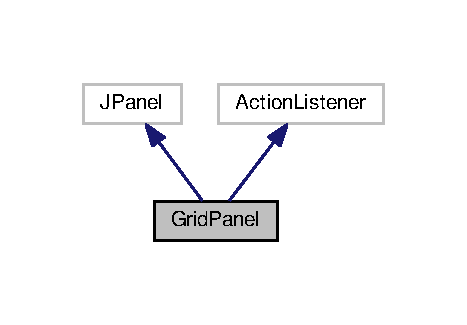
\includegraphics[width=224pt]{classGridPanel__inherit__graph}
\end{center}
\end{figure}


Collaboration diagram for Grid\+Panel\+:\nopagebreak
\begin{figure}[H]
\begin{center}
\leavevmode
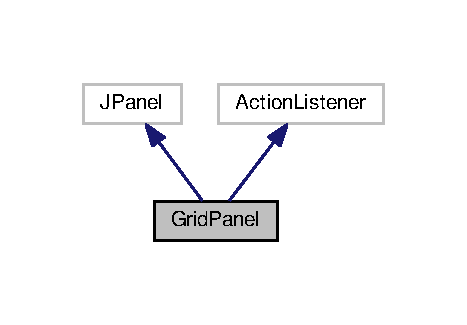
\includegraphics[width=224pt]{classGridPanel__coll__graph}
\end{center}
\end{figure}
\subsection*{Public Member Functions}
\begin{DoxyCompactItemize}
\item 
\hyperlink{classGridPanel_af8bf9b3bb5b5548a39f97371848e0ac7}{Grid\+Panel} (int width, int height, \hyperlink{classUser}{User} player, \hyperlink{classGame}{Game} game, J\+Panel card\+Layout\+Panel)
\begin{DoxyCompactList}\small\item\em Constructor. \end{DoxyCompactList}\item 
\hyperlink{classGUIListener}{G\+U\+I\+Listener} {\bfseries get\+Listener} ()\hypertarget{classGridPanel_a297c91de7bf845e66bd2ae03c1635950}{}\label{classGridPanel_a297c91de7bf845e66bd2ae03c1635950}

\item 
\hyperlink{classGame}{Game} {\bfseries get\+Game} ()\hypertarget{classGridPanel_a2eb320db357aef01be7b27ecf045bbbf}{}\label{classGridPanel_a2eb320db357aef01be7b27ecf045bbbf}

\item 
boolean {\bfseries is\+Ready} ()\hypertarget{classGridPanel_aae632b11eaed927afd5884f99a5870f8}{}\label{classGridPanel_aae632b11eaed927afd5884f99a5870f8}

\item 
void {\bfseries set\+Ready} (boolean ready)\hypertarget{classGridPanel_a09c32b26eae81ac799aa95e28aae194f}{}\label{classGridPanel_a09c32b26eae81ac799aa95e28aae194f}

\item 
J\+Panel {\bfseries get\+Card\+Layout\+Panel} ()\hypertarget{classGridPanel_a1a8601fc7d4f8175c7aebd6bec8ec6f9}{}\label{classGridPanel_a1a8601fc7d4f8175c7aebd6bec8ec6f9}

\item 
void \hyperlink{classGridPanel_a38f9375b4ed14fa70edaa859b0ed43e6}{action\+Performed} (Action\+Event action\+Event)\hypertarget{classGridPanel_a38f9375b4ed14fa70edaa859b0ed43e6}{}\label{classGridPanel_a38f9375b4ed14fa70edaa859b0ed43e6}

\begin{DoxyCompactList}\small\item\em Repaint each move. \end{DoxyCompactList}\item 
String {\bfseries to\+String} ()\hypertarget{classGridPanel_a7dbc1ff2bf786538707f479837ce2792}{}\label{classGridPanel_a7dbc1ff2bf786538707f479837ce2792}

\end{DoxyCompactItemize}
\subsection*{Public Attributes}
\begin{DoxyCompactItemize}
\item 
final int {\bfseries W\+I\+D\+TH}\hypertarget{classGridPanel_a0ad964f4019fe73ca89797e3b2ba6801}{}\label{classGridPanel_a0ad964f4019fe73ca89797e3b2ba6801}

\item 
final int {\bfseries H\+E\+I\+G\+HT}\hypertarget{classGridPanel_a1a9b96aea68e7aa0b30ae9663760bb97}{}\label{classGridPanel_a1a9b96aea68e7aa0b30ae9663760bb97}

\end{DoxyCompactItemize}
\subsection*{Protected Member Functions}
\begin{DoxyCompactItemize}
\item 
void \hyperlink{classGridPanel_ae44d617ba15ff9b1778cc4c713151650}{paint\+Component} (Graphics g)\hypertarget{classGridPanel_ae44d617ba15ff9b1778cc4c713151650}{}\label{classGridPanel_ae44d617ba15ff9b1778cc4c713151650}

\begin{DoxyCompactList}\small\item\em Draw the board. \end{DoxyCompactList}\end{DoxyCompactItemize}


\subsection{Detailed Description}
Panel representing board. 

\subsection{Constructor \& Destructor Documentation}
\index{Grid\+Panel@{Grid\+Panel}!Grid\+Panel@{Grid\+Panel}}
\index{Grid\+Panel@{Grid\+Panel}!Grid\+Panel@{Grid\+Panel}}
\subsubsection[{\texorpdfstring{Grid\+Panel(int width, int height, User player, Game game, J\+Panel card\+Layout\+Panel)}{GridPanel(int width, int height, User player, Game game, JPanel cardLayoutPanel)}}]{\setlength{\rightskip}{0pt plus 5cm}Grid\+Panel.\+Grid\+Panel (
\begin{DoxyParamCaption}
\item[{int}]{width, }
\item[{int}]{height, }
\item[{{\bf User}}]{player, }
\item[{{\bf Game}}]{game, }
\item[{J\+Panel}]{card\+Layout\+Panel}
\end{DoxyParamCaption}
)\hspace{0.3cm}{\ttfamily [inline]}}\hypertarget{classGridPanel_af8bf9b3bb5b5548a39f97371848e0ac7}{}\label{classGridPanel_af8bf9b3bb5b5548a39f97371848e0ac7}


Constructor. 


\begin{DoxyParams}{Parameters}
{\em width} & width of panel. \\
\hline
{\em height} & height of panel. \\
\hline
{\em player} & \hyperlink{classPlayer}{Player} object. \\
\hline
{\em game} & \hyperlink{classGame}{Game} object. \\
\hline
{\em card\+Layout\+Panel} & J\+Panel having Card\+Layout. \\
\hline
\end{DoxyParams}


The documentation for this class was generated from the following file\+:\begin{DoxyCompactItemize}
\item 
src/Grid\+Panel.\+java\end{DoxyCompactItemize}

\hypertarget{classGUIListener}{}\section{G\+U\+I\+Listener Class Reference}
\label{classGUIListener}\index{G\+U\+I\+Listener@{G\+U\+I\+Listener}}


Inheritance diagram for G\+U\+I\+Listener\+:
\nopagebreak
\begin{figure}[H]
\begin{center}
\leavevmode
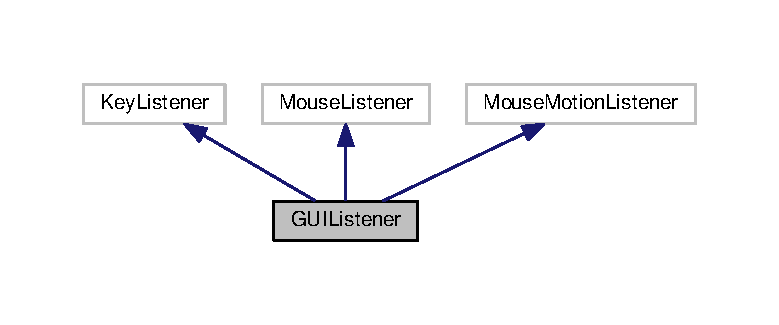
\includegraphics[width=350pt]{classGUIListener__inherit__graph}
\end{center}
\end{figure}


Collaboration diagram for G\+U\+I\+Listener\+:
\nopagebreak
\begin{figure}[H]
\begin{center}
\leavevmode
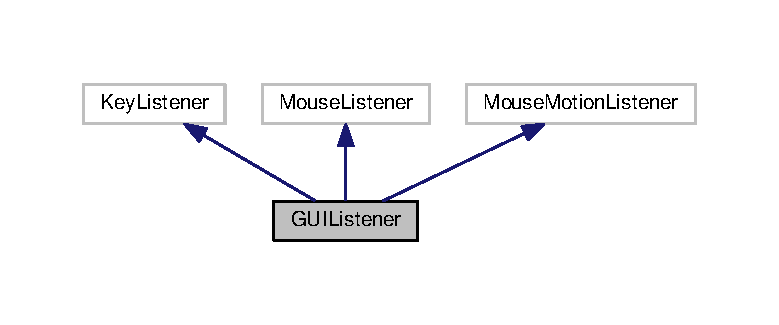
\includegraphics[width=350pt]{classGUIListener__coll__graph}
\end{center}
\end{figure}
\subsection*{Public Member Functions}
\begin{DoxyCompactItemize}
\item 
{\bfseries G\+U\+I\+Listener} (int width, int height, \hyperlink{classGame}{Game} game, \hyperlink{classPlayer}{Player} player, \hyperlink{classGridPanel}{Grid\+Panel} panel)\hypertarget{classGUIListener_af4885004ac07dbdcc72cde2b7c0cde14}{}\label{classGUIListener_af4885004ac07dbdcc72cde2b7c0cde14}

\item 
boolean {\bfseries is\+Horizontal} ()\hypertarget{classGUIListener_af6a1761ae16169e68eadc58cf7051bea}{}\label{classGUIListener_af6a1761ae16169e68eadc58cf7051bea}

\item 
int {\bfseries get\+MouseX} ()\hypertarget{classGUIListener_a11a624deb04ae126517f37e6b1883aad}{}\label{classGUIListener_a11a624deb04ae126517f37e6b1883aad}

\item 
int {\bfseries get\+MouseY} ()\hypertarget{classGUIListener_ad8f1ceb49938fc6c5869202ac1383b74}{}\label{classGUIListener_ad8f1ceb49938fc6c5869202ac1383b74}

\item 
int {\bfseries get\+Ship\+Size} ()\hypertarget{classGUIListener_a4c107528ebd4f160674ecbaf9b125bf9}{}\label{classGUIListener_a4c107528ebd4f160674ecbaf9b125bf9}

\item 
boolean {\bfseries is\+Active} ()\hypertarget{classGUIListener_a0559c02a1f4b20ba00b3195d76de05d4}{}\label{classGUIListener_a0559c02a1f4b20ba00b3195d76de05d4}

\item 
void {\bfseries set\+Active} (boolean active)\hypertarget{classGUIListener_a2834f4c5089485e247184aba22ffa36e}{}\label{classGUIListener_a2834f4c5089485e247184aba22ffa36e}

\item 
void {\bfseries mouse\+Clicked} (Mouse\+Event mouse\+Event)\hypertarget{classGUIListener_ab0cfe7af17bab2decc326dc1a0b0373b}{}\label{classGUIListener_ab0cfe7af17bab2decc326dc1a0b0373b}

\item 
void {\bfseries mouse\+Pressed} (Mouse\+Event mouse\+Event)\hypertarget{classGUIListener_a924b03b8a466f02543597017825c92a0}{}\label{classGUIListener_a924b03b8a466f02543597017825c92a0}

\item 
void {\bfseries mouse\+Released} (Mouse\+Event mouse\+Event)\hypertarget{classGUIListener_ad9d4c366f5e965a2859d34008021296e}{}\label{classGUIListener_ad9d4c366f5e965a2859d34008021296e}

\item 
void {\bfseries mouse\+Entered} (Mouse\+Event mouse\+Event)\hypertarget{classGUIListener_a3a714ed0ff377a41d830a884adfe20e5}{}\label{classGUIListener_a3a714ed0ff377a41d830a884adfe20e5}

\item 
void {\bfseries mouse\+Exited} (Mouse\+Event mouse\+Event)\hypertarget{classGUIListener_aa4038ada664a15857dc2dea6ef19361c}{}\label{classGUIListener_aa4038ada664a15857dc2dea6ef19361c}

\item 
void {\bfseries mouse\+Dragged} (Mouse\+Event mouse\+Event)\hypertarget{classGUIListener_a03270bb04cc49e7cc40a07cec897a03d}{}\label{classGUIListener_a03270bb04cc49e7cc40a07cec897a03d}

\item 
void {\bfseries mouse\+Moved} (Mouse\+Event mouse\+Event)\hypertarget{classGUIListener_acfd39f94b381ec2fd3653bb18137a3a0}{}\label{classGUIListener_acfd39f94b381ec2fd3653bb18137a3a0}

\item 
void {\bfseries key\+Typed} (Key\+Event key\+Event)\hypertarget{classGUIListener_a7aacf142d63f4ef87009903be279ad70}{}\label{classGUIListener_a7aacf142d63f4ef87009903be279ad70}

\item 
void {\bfseries key\+Pressed} (Key\+Event key\+Event)\hypertarget{classGUIListener_a469eaac915f1d10930dcdde8feec3fb5}{}\label{classGUIListener_a469eaac915f1d10930dcdde8feec3fb5}

\item 
void {\bfseries key\+Released} (Key\+Event key\+Event)\hypertarget{classGUIListener_a0384d5954bf3864eeafd989d34f102ad}{}\label{classGUIListener_a0384d5954bf3864eeafd989d34f102ad}

\end{DoxyCompactItemize}


The documentation for this class was generated from the following file\+:\begin{DoxyCompactItemize}
\item 
src/G\+U\+I\+Listener.\+java\end{DoxyCompactItemize}

\hypertarget{classMain}{}\section{Main Class Reference}
\label{classMain}\index{Main@{Main}}


\hyperlink{classMain}{Main} class to run a game.  


\subsection*{Static Public Member Functions}
\begin{DoxyCompactItemize}
\item 
static void \hyperlink{classMain_a8a5d0f827edddff706cc0e6740d0579a}{main} (String\mbox{[}$\,$\mbox{]} args)  throws I\+O\+Exception \hypertarget{classMain_a8a5d0f827edddff706cc0e6740d0579a}{}\label{classMain_a8a5d0f827edddff706cc0e6740d0579a}

\begin{DoxyCompactList}\small\item\em Starting point of a game. \end{DoxyCompactList}\end{DoxyCompactItemize}


\subsection{Detailed Description}
\hyperlink{classMain}{Main} class to run a game. 

The documentation for this class was generated from the following file\+:\begin{DoxyCompactItemize}
\item 
src/Main.\+java\end{DoxyCompactItemize}

\hypertarget{classMainGUI}{}\section{Main\+G\+UI Class Reference}
\label{classMainGUI}\index{Main\+G\+UI@{Main\+G\+UI}}


\hyperlink{classMain}{Main} class.  


\subsection*{Public Member Functions}
\begin{DoxyCompactItemize}
\item 
\hyperlink{classMainGUI_a49c09db8105ae715258f1a29ac318c66}{Main\+G\+UI} ()
\begin{DoxyCompactList}\small\item\em Constructor. \end{DoxyCompactList}\item 
int \hyperlink{classMainGUI_a3d35950de747333a96fa0cca3c38eff5}{get\+Start} ()
\begin{DoxyCompactList}\small\item\em Getter for start. \end{DoxyCompactList}\item 
void \hyperlink{classMainGUI_abefcabebf411d9ae06fd1bd0c979ab59}{set\+Start} (int start)
\begin{DoxyCompactList}\small\item\em Setter for start. \end{DoxyCompactList}\end{DoxyCompactItemize}
\subsection*{Static Public Member Functions}
\begin{DoxyCompactItemize}
\item 
static void \hyperlink{classMainGUI_a8dd5b61b10beb51baab3664b296c4381}{main} (String\mbox{[}$\,$\mbox{]} args)\hypertarget{classMainGUI_a8dd5b61b10beb51baab3664b296c4381}{}\label{classMainGUI_a8dd5b61b10beb51baab3664b296c4381}

\begin{DoxyCompactList}\small\item\em Starting point of a game. \end{DoxyCompactList}\end{DoxyCompactItemize}
\subsection*{Static Public Attributes}
\begin{DoxyCompactItemize}
\item 
static final int {\bfseries W\+I\+D\+TH} = 1050\hypertarget{classMainGUI_a3bdc2df4130838ec598e0b04abd21867}{}\label{classMainGUI_a3bdc2df4130838ec598e0b04abd21867}

\item 
static final int {\bfseries H\+E\+I\+G\+HT} = 500\hypertarget{classMainGUI_aa09eba3beefdff644cbedca2cee85cdd}{}\label{classMainGUI_aa09eba3beefdff644cbedca2cee85cdd}

\end{DoxyCompactItemize}


\subsection{Detailed Description}
\hyperlink{classMain}{Main} class. 

Class that runs a game. 

\subsection{Constructor \& Destructor Documentation}
\index{Main\+G\+UI@{Main\+G\+UI}!Main\+G\+UI@{Main\+G\+UI}}
\index{Main\+G\+UI@{Main\+G\+UI}!Main\+G\+UI@{Main\+G\+UI}}
\subsubsection[{\texorpdfstring{Main\+G\+U\+I()}{MainGUI()}}]{\setlength{\rightskip}{0pt plus 5cm}Main\+G\+U\+I.\+Main\+G\+UI (
\begin{DoxyParamCaption}
{}
\end{DoxyParamCaption}
)\hspace{0.3cm}{\ttfamily [inline]}}\hypertarget{classMainGUI_a49c09db8105ae715258f1a29ac318c66}{}\label{classMainGUI_a49c09db8105ae715258f1a29ac318c66}


Constructor. 

Creates panels and runs a game. 

\subsection{Member Function Documentation}
\index{Main\+G\+UI@{Main\+G\+UI}!get\+Start@{get\+Start}}
\index{get\+Start@{get\+Start}!Main\+G\+UI@{Main\+G\+UI}}
\subsubsection[{\texorpdfstring{get\+Start()}{getStart()}}]{\setlength{\rightskip}{0pt plus 5cm}int Main\+G\+U\+I.\+get\+Start (
\begin{DoxyParamCaption}
{}
\end{DoxyParamCaption}
)\hspace{0.3cm}{\ttfamily [inline]}}\hypertarget{classMainGUI_a3d35950de747333a96fa0cca3c38eff5}{}\label{classMainGUI_a3d35950de747333a96fa0cca3c38eff5}


Getter for start. 

\begin{DoxyReturn}{Returns}
value of start. 
\end{DoxyReturn}
\index{Main\+G\+UI@{Main\+G\+UI}!set\+Start@{set\+Start}}
\index{set\+Start@{set\+Start}!Main\+G\+UI@{Main\+G\+UI}}
\subsubsection[{\texorpdfstring{set\+Start(int start)}{setStart(int start)}}]{\setlength{\rightskip}{0pt plus 5cm}void Main\+G\+U\+I.\+set\+Start (
\begin{DoxyParamCaption}
\item[{int}]{start}
\end{DoxyParamCaption}
)\hspace{0.3cm}{\ttfamily [inline]}}\hypertarget{classMainGUI_abefcabebf411d9ae06fd1bd0c979ab59}{}\label{classMainGUI_abefcabebf411d9ae06fd1bd0c979ab59}


Setter for start. 


\begin{DoxyParams}{Parameters}
{\em start} & value of start. \\
\hline
\end{DoxyParams}


The documentation for this class was generated from the following file\+:\begin{DoxyCompactItemize}
\item 
src/Main\+G\+U\+I.\+java\end{DoxyCompactItemize}

\hypertarget{classMainMenuPanel}{}\section{Main\+Menu\+Panel Class Reference}
\label{classMainMenuPanel}\index{Main\+Menu\+Panel@{Main\+Menu\+Panel}}


Panel of main menu.  




Inheritance diagram for Main\+Menu\+Panel\+:
\nopagebreak
\begin{figure}[H]
\begin{center}
\leavevmode
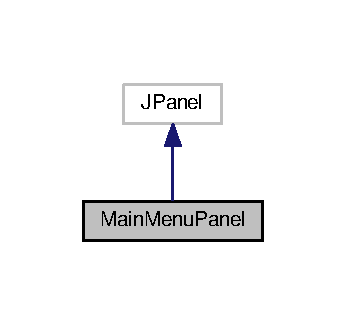
\includegraphics[width=166pt]{classMainMenuPanel__inherit__graph}
\end{center}
\end{figure}


Collaboration diagram for Main\+Menu\+Panel\+:
\nopagebreak
\begin{figure}[H]
\begin{center}
\leavevmode
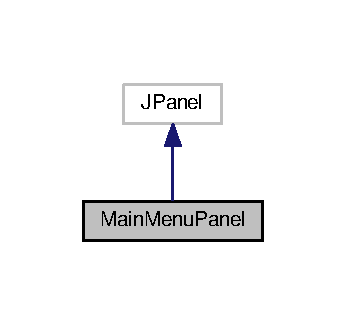
\includegraphics[width=166pt]{classMainMenuPanel__coll__graph}
\end{center}
\end{figure}
\subsection*{Public Member Functions}
\begin{DoxyCompactItemize}
\item 
\hyperlink{classMainMenuPanel_a84d6e512c79963a1a77aaa48fa3c0211}{Main\+Menu\+Panel} (int width, int height, \hyperlink{classMainGUI}{Main\+G\+UI} runner)
\begin{DoxyCompactList}\small\item\em Constructor. \end{DoxyCompactList}\end{DoxyCompactItemize}
\subsection*{Public Attributes}
\begin{DoxyCompactItemize}
\item 
final int {\bfseries W\+I\+D\+TH}\hypertarget{classMainMenuPanel_a40a16a0906506f77e058246871edb7aa}{}\label{classMainMenuPanel_a40a16a0906506f77e058246871edb7aa}

\item 
final int {\bfseries H\+E\+I\+G\+HT}\hypertarget{classMainMenuPanel_a16cccb47e75566ec2d0a619390ce791a}{}\label{classMainMenuPanel_a16cccb47e75566ec2d0a619390ce791a}

\end{DoxyCompactItemize}
\subsection*{Protected Member Functions}
\begin{DoxyCompactItemize}
\item 
void \hyperlink{classMainMenuPanel_a912f66021f4771dfb4bac2150c18ffc6}{paint\+Component} (Graphics g)\hypertarget{classMainMenuPanel_a912f66021f4771dfb4bac2150c18ffc6}{}\label{classMainMenuPanel_a912f66021f4771dfb4bac2150c18ffc6}

\begin{DoxyCompactList}\small\item\em Draw the background. \end{DoxyCompactList}\end{DoxyCompactItemize}


\subsection{Detailed Description}
Panel of main menu. 

Class representing a main menu panel. 

\subsection{Constructor \& Destructor Documentation}
\index{Main\+Menu\+Panel@{Main\+Menu\+Panel}!Main\+Menu\+Panel@{Main\+Menu\+Panel}}
\index{Main\+Menu\+Panel@{Main\+Menu\+Panel}!Main\+Menu\+Panel@{Main\+Menu\+Panel}}
\subsubsection[{\texorpdfstring{Main\+Menu\+Panel(int width, int height, Main\+G\+U\+I runner)}{MainMenuPanel(int width, int height, MainGUI runner)}}]{\setlength{\rightskip}{0pt plus 5cm}Main\+Menu\+Panel.\+Main\+Menu\+Panel (
\begin{DoxyParamCaption}
\item[{int}]{width, }
\item[{int}]{height, }
\item[{{\bf Main\+G\+UI}}]{runner}
\end{DoxyParamCaption}
)\hspace{0.3cm}{\ttfamily [inline]}}\hypertarget{classMainMenuPanel_a84d6e512c79963a1a77aaa48fa3c0211}{}\label{classMainMenuPanel_a84d6e512c79963a1a77aaa48fa3c0211}


Constructor. 


\begin{DoxyParams}{Parameters}
{\em width} & width of panel. \\
\hline
{\em height} & height of panel. \\
\hline
{\em runner} & \hyperlink{classMainGUI}{Main\+G\+UI} object creating the panel. \\
\hline
\end{DoxyParams}


The documentation for this class was generated from the following file\+:\begin{DoxyCompactItemize}
\item 
src/Main\+Menu\+Panel.\+java\end{DoxyCompactItemize}

\hypertarget{classPlayer}{}\section{Player Class Reference}
\label{classPlayer}\index{Player@{Player}}


\hyperlink{classPlayer}{Player} abstract class.  




Inheritance diagram for Player\+:
\nopagebreak
\begin{figure}[H]
\begin{center}
\leavevmode
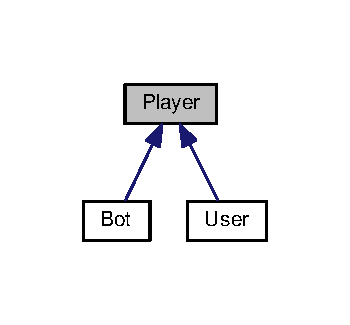
\includegraphics[width=168pt]{classPlayer__inherit__graph}
\end{center}
\end{figure}
\subsection*{Public Member Functions}
\begin{DoxyCompactItemize}
\item 
\hyperlink{classPlayer_a0444e17b6e068f2cbee6937244c8f921}{Player} (\hyperlink{classGame}{Game} game, int id)
\begin{DoxyCompactList}\small\item\em Constructor. \end{DoxyCompactList}\item 
\hyperlink{classShip}{Ship}\mbox{[}$\,$\mbox{]} {\bfseries get\+Ships} ()\hypertarget{classPlayer_a992bcaa016d561372f176b0021b624d2}{}\label{classPlayer_a992bcaa016d561372f176b0021b624d2}

\item 
\hyperlink{classShip}{Ship} {\bfseries get\+Ship} (int index)\hypertarget{classPlayer_af2d7d0a6c12ccb105fedf289516463ca}{}\label{classPlayer_af2d7d0a6c12ccb105fedf289516463ca}

\item 
char\mbox{[}$\,$\mbox{]}\mbox{[}$\,$\mbox{]} {\bfseries get\+Grid\+Mine} ()\hypertarget{classPlayer_ae9eb4d4e55b285791cdfa946f33042ae}{}\label{classPlayer_ae9eb4d4e55b285791cdfa946f33042ae}

\item 
char {\bfseries get\+Grid\+Mine} (int x, int y)\hypertarget{classPlayer_aee4d0aabd398122c3406d9a193d2fc33}{}\label{classPlayer_aee4d0aabd398122c3406d9a193d2fc33}

\item 
char\mbox{[}$\,$\mbox{]}\mbox{[}$\,$\mbox{]} {\bfseries get\+Grid\+Opponent} ()\hypertarget{classPlayer_ae8c3f7b3895e4d8f5e96f5f072bf7211}{}\label{classPlayer_ae8c3f7b3895e4d8f5e96f5f072bf7211}

\item 
char {\bfseries get\+Grid\+Opponent} (int x, int y)\hypertarget{classPlayer_ab82aed9ca2e326d51614a6287dd355d9}{}\label{classPlayer_ab82aed9ca2e326d51614a6287dd355d9}

\item 
\hyperlink{classGame}{Game} {\bfseries get\+Game} ()\hypertarget{classPlayer_a08580623035eedb19e8b7a028ad64914}{}\label{classPlayer_a08580623035eedb19e8b7a028ad64914}

\item 
int {\bfseries get\+Id} ()\hypertarget{classPlayer_adea0e90dc94ac68c20d672f801dc951a}{}\label{classPlayer_adea0e90dc94ac68c20d672f801dc951a}

\item 
void {\bfseries set\+Ships} (\hyperlink{classShip}{Ship}\mbox{[}$\,$\mbox{]} ships)\hypertarget{classPlayer_ae4027662c9c93b5c023838a36a303a04}{}\label{classPlayer_ae4027662c9c93b5c023838a36a303a04}

\item 
void {\bfseries set\+Ship} (int index, \hyperlink{classShip}{Ship} ship)\hypertarget{classPlayer_a3235c3e8a2434947ebe9748abed80fda}{}\label{classPlayer_a3235c3e8a2434947ebe9748abed80fda}

\item 
void {\bfseries set\+Grid\+Mine} (char\mbox{[}$\,$\mbox{]}\mbox{[}$\,$\mbox{]} grid\+Mine)\hypertarget{classPlayer_affa3bbe73b17f997591a92aaf6d8da33}{}\label{classPlayer_affa3bbe73b17f997591a92aaf6d8da33}

\item 
void {\bfseries set\+Grid\+Mine} (int x, int y, char val)\hypertarget{classPlayer_a8f3ce6a037eabdb592f421b77948af27}{}\label{classPlayer_a8f3ce6a037eabdb592f421b77948af27}

\item 
void {\bfseries set\+Grid\+Opponent} (char\mbox{[}$\,$\mbox{]}\mbox{[}$\,$\mbox{]} grid\+Opponent)\hypertarget{classPlayer_a3b65aecb541790ce379f68828a24517a}{}\label{classPlayer_a3b65aecb541790ce379f68828a24517a}

\item 
void {\bfseries set\+Grid\+Opponent} (int x, int y, char val)\hypertarget{classPlayer_a9555543f75989387be2e65769fbba816}{}\label{classPlayer_a9555543f75989387be2e65769fbba816}

\item 
void {\bfseries set\+Game} (\hyperlink{classGame}{Game} game)\hypertarget{classPlayer_a75ac90ea1583ab7f6b09c48f7f414f44}{}\label{classPlayer_a75ac90ea1583ab7f6b09c48f7f414f44}

\item 
boolean {\bfseries is\+Ready} ()\hypertarget{classPlayer_a25d2009e1520e66fa0afed74111e1e7f}{}\label{classPlayer_a25d2009e1520e66fa0afed74111e1e7f}

\item 
void {\bfseries set\+Ready} (boolean ready)\hypertarget{classPlayer_a05b0f61d5105e6f759e902aa84c30630}{}\label{classPlayer_a05b0f61d5105e6f759e902aa84c30630}

\item 
abstract void \hyperlink{classPlayer_ac9db31c39141ff98362287a8bb998ef4}{build\+Ships} ()\hypertarget{classPlayer_ac9db31c39141ff98362287a8bb998ef4}{}\label{classPlayer_ac9db31c39141ff98362287a8bb998ef4}

\begin{DoxyCompactList}\small\item\em Abstract method to build \hyperlink{classShip}{Ship}\textquotesingle{}s. \end{DoxyCompactList}\item 
abstract void \hyperlink{classPlayer_abd852c2c1a9728644a45dd53a84871de}{attack} ()\hypertarget{classPlayer_abd852c2c1a9728644a45dd53a84871de}{}\label{classPlayer_abd852c2c1a9728644a45dd53a84871de}

\begin{DoxyCompactList}\small\item\em Abstract method to attack the opponent\textquotesingle{}s \hyperlink{classShip}{Ship}\textquotesingle{}s. \end{DoxyCompactList}\item 
boolean \hyperlink{classPlayer_a21c42ba135673c82075eebb3f9ea6d5c}{attempt\+To\+Build} (int x, int y, int segment\+Num, boolean is\+Horizontal)
\begin{DoxyCompactList}\small\item\em Attempt to build a segment\+Num-\/segment \hyperlink{classShip}{Ship} at given (x, y) with given orientation. \end{DoxyCompactList}\item 
void \hyperlink{classPlayer_ae551f266c116f22887d278f6beaf9e75}{show\+Grid\+Mine} (boolean clear)
\begin{DoxyCompactList}\small\item\em Show player\textquotesingle{}s grid. \end{DoxyCompactList}\item 
void \hyperlink{classPlayer_ade7e5623438ad21421091dcc201b367c}{show\+Grid\+Opponent} (boolean clear)
\begin{DoxyCompactList}\small\item\em Show opponent\textquotesingle{}s grid. \end{DoxyCompactList}\item 
void \hyperlink{classPlayer_ad571760f9739182566e3817e515fd3c1}{show\+Grids} (boolean clear)
\begin{DoxyCompactList}\small\item\em Show player\textquotesingle{}s and opponent\textquotesingle{}s grids. \end{DoxyCompactList}\item 
int \hyperlink{classPlayer_ac4e41793e0e2fd8cfaabad6775cdfaa0}{get\+Damage} (int x, int y)
\begin{DoxyCompactList}\small\item\em Get damage at given (x, y). \end{DoxyCompactList}\end{DoxyCompactItemize}


\subsection{Detailed Description}
\hyperlink{classPlayer}{Player} abstract class. 

Implements the idea of a player in a game. 

\subsection{Constructor \& Destructor Documentation}
\index{Player@{Player}!Player@{Player}}
\index{Player@{Player}!Player@{Player}}
\subsubsection[{\texorpdfstring{Player(\+Game game, int id)}{Player(Game game, int id)}}]{\setlength{\rightskip}{0pt plus 5cm}Player.\+Player (
\begin{DoxyParamCaption}
\item[{{\bf Game}}]{game, }
\item[{int}]{id}
\end{DoxyParamCaption}
)\hspace{0.3cm}{\ttfamily [inline]}}\hypertarget{classPlayer_a0444e17b6e068f2cbee6937244c8f921}{}\label{classPlayer_a0444e17b6e068f2cbee6937244c8f921}


Constructor. 


\begin{DoxyParams}{Parameters}
{\em game} & \hyperlink{classGame}{Game} object. \\
\hline
{\em id} & Id of a player. \\
\hline
\end{DoxyParams}


\subsection{Member Function Documentation}
\index{Player@{Player}!attempt\+To\+Build@{attempt\+To\+Build}}
\index{attempt\+To\+Build@{attempt\+To\+Build}!Player@{Player}}
\subsubsection[{\texorpdfstring{attempt\+To\+Build(int x, int y, int segment\+Num, boolean is\+Horizontal)}{attemptToBuild(int x, int y, int segmentNum, boolean isHorizontal)}}]{\setlength{\rightskip}{0pt plus 5cm}boolean Player.\+attempt\+To\+Build (
\begin{DoxyParamCaption}
\item[{int}]{x, }
\item[{int}]{y, }
\item[{int}]{segment\+Num, }
\item[{boolean}]{is\+Horizontal}
\end{DoxyParamCaption}
)\hspace{0.3cm}{\ttfamily [inline]}}\hypertarget{classPlayer_a21c42ba135673c82075eebb3f9ea6d5c}{}\label{classPlayer_a21c42ba135673c82075eebb3f9ea6d5c}


Attempt to build a segment\+Num-\/segment \hyperlink{classShip}{Ship} at given (x, y) with given orientation. 


\begin{DoxyParams}{Parameters}
{\em x} & x-\/coordinate. \\
\hline
{\em y} & y-\/coordinate. \\
\hline
{\em segment\+Num} & number of segments of a \hyperlink{classShip}{Ship} object. \\
\hline
{\em is\+Horizontal} & boolean representing an orientation of a \hyperlink{classShip}{Ship} object. \\
\hline
\end{DoxyParams}
\begin{DoxyReturn}{Returns}

\end{DoxyReturn}
\index{Player@{Player}!get\+Damage@{get\+Damage}}
\index{get\+Damage@{get\+Damage}!Player@{Player}}
\subsubsection[{\texorpdfstring{get\+Damage(int x, int y)}{getDamage(int x, int y)}}]{\setlength{\rightskip}{0pt plus 5cm}int Player.\+get\+Damage (
\begin{DoxyParamCaption}
\item[{int}]{x, }
\item[{int}]{y}
\end{DoxyParamCaption}
)\hspace{0.3cm}{\ttfamily [inline]}}\hypertarget{classPlayer_ac4e41793e0e2fd8cfaabad6775cdfaa0}{}\label{classPlayer_ac4e41793e0e2fd8cfaabad6775cdfaa0}


Get damage at given (x, y). 


\begin{DoxyParams}{Parameters}
{\em x} & x-\/coordinate. \\
\hline
{\em y} & y-\/coordinate. \\
\hline
\end{DoxyParams}
\begin{DoxyReturn}{Returns}
H\+IT in the case of a hit, S\+I\+NK in the case of sink. 
\end{DoxyReturn}
\index{Player@{Player}!show\+Grid\+Mine@{show\+Grid\+Mine}}
\index{show\+Grid\+Mine@{show\+Grid\+Mine}!Player@{Player}}
\subsubsection[{\texorpdfstring{show\+Grid\+Mine(boolean clear)}{showGridMine(boolean clear)}}]{\setlength{\rightskip}{0pt plus 5cm}void Player.\+show\+Grid\+Mine (
\begin{DoxyParamCaption}
\item[{boolean}]{clear}
\end{DoxyParamCaption}
)\hspace{0.3cm}{\ttfamily [inline]}}\hypertarget{classPlayer_ae551f266c116f22887d278f6beaf9e75}{}\label{classPlayer_ae551f266c116f22887d278f6beaf9e75}


Show player\textquotesingle{}s grid. 


\begin{DoxyParams}{Parameters}
{\em clear} & boolean specifying whether to clean a terminal before showing a grid. \\
\hline
\end{DoxyParams}
\index{Player@{Player}!show\+Grid\+Opponent@{show\+Grid\+Opponent}}
\index{show\+Grid\+Opponent@{show\+Grid\+Opponent}!Player@{Player}}
\subsubsection[{\texorpdfstring{show\+Grid\+Opponent(boolean clear)}{showGridOpponent(boolean clear)}}]{\setlength{\rightskip}{0pt plus 5cm}void Player.\+show\+Grid\+Opponent (
\begin{DoxyParamCaption}
\item[{boolean}]{clear}
\end{DoxyParamCaption}
)\hspace{0.3cm}{\ttfamily [inline]}}\hypertarget{classPlayer_ade7e5623438ad21421091dcc201b367c}{}\label{classPlayer_ade7e5623438ad21421091dcc201b367c}


Show opponent\textquotesingle{}s grid. 


\begin{DoxyParams}{Parameters}
{\em clear} & boolean specifying whether to clean a terminal before showing a grid. \\
\hline
\end{DoxyParams}
\index{Player@{Player}!show\+Grids@{show\+Grids}}
\index{show\+Grids@{show\+Grids}!Player@{Player}}
\subsubsection[{\texorpdfstring{show\+Grids(boolean clear)}{showGrids(boolean clear)}}]{\setlength{\rightskip}{0pt plus 5cm}void Player.\+show\+Grids (
\begin{DoxyParamCaption}
\item[{boolean}]{clear}
\end{DoxyParamCaption}
)\hspace{0.3cm}{\ttfamily [inline]}}\hypertarget{classPlayer_ad571760f9739182566e3817e515fd3c1}{}\label{classPlayer_ad571760f9739182566e3817e515fd3c1}


Show player\textquotesingle{}s and opponent\textquotesingle{}s grids. 


\begin{DoxyParams}{Parameters}
{\em clear} & boolean specifying whether to clean a terminal before showing grids. \\
\hline
\end{DoxyParams}


The documentation for this class was generated from the following file\+:\begin{DoxyCompactItemize}
\item 
src/Player.\+java\end{DoxyCompactItemize}

\hypertarget{classShip}{}\section{Ship Class Reference}
\label{classShip}\index{Ship@{Ship}}


\hyperlink{classShip}{Ship} class.  


\subsection*{Public Member Functions}
\begin{DoxyCompactItemize}
\item 
\hyperlink{classShip_aad9f864d03a4d6e4410ef058a07a887d}{Ship} (int x, int y, int segment\+Num, boolean is\+Horizontal)
\begin{DoxyCompactList}\small\item\em Constructor. \end{DoxyCompactList}\item 
int \hyperlink{classShip_a1cb1ffc138ae22488954a8f9cbd7a227}{getX} ()
\begin{DoxyCompactList}\small\item\em Getter for x. \end{DoxyCompactList}\item 
int \hyperlink{classShip_a7dd07d0fdb652e1ce70f2442d6b1171c}{getY} ()
\begin{DoxyCompactList}\small\item\em Getter for y. \end{DoxyCompactList}\item 
boolean \hyperlink{classShip_a5931f11cfaaecf82200263373d777249}{is\+Horizontal} ()
\begin{DoxyCompactList}\small\item\em Getter for orientation of a ship. \end{DoxyCompactList}\item 
boolean\mbox{[}$\,$\mbox{]} \hyperlink{classShip_ab18527e0957bdb9a286a91fea5bfd500}{get\+Health} ()
\begin{DoxyCompactList}\small\item\em Getter for HP. \end{DoxyCompactList}\item 
void \hyperlink{classShip_ae5dfe53a340d63db1dfcda3d43138775}{setX} (int x)
\begin{DoxyCompactList}\small\item\em Setter for x. \end{DoxyCompactList}\item 
void \hyperlink{classShip_a8b4bd2064164d6310f2035249b5c2e8d}{setY} (int y)
\begin{DoxyCompactList}\small\item\em Setter for y. \end{DoxyCompactList}\item 
void \hyperlink{classShip_a170cbc736f06285b709a3d110b0f3da9}{set\+Horizontal} (boolean horizontal)
\begin{DoxyCompactList}\small\item\em Setter for orientation. \end{DoxyCompactList}\item 
void \hyperlink{classShip_af1524176d95bdcd4699606020f491a36}{set\+Health} (boolean\mbox{[}$\,$\mbox{]} health)
\begin{DoxyCompactList}\small\item\em Setter for HP. \end{DoxyCompactList}\item 
void \hyperlink{classShip_ab7049cd23905649a2b382a8e1f022baf}{get\+Damage} (int x, int y)
\begin{DoxyCompactList}\small\item\em Get damage at given (x, y) coordinates. \end{DoxyCompactList}\item 
boolean \hyperlink{classShip_a60e1c5cd27f8779cdd668580bc76fb2f}{is\+Dead} ()
\begin{DoxyCompactList}\small\item\em Is a ship sunk? \end{DoxyCompactList}\item 
boolean \hyperlink{classShip_a4a9ded86f4c02bb9ab8936314dd228aa}{is\+At} (int x, int y)
\begin{DoxyCompactList}\small\item\em Is a ship at (x, y)? \end{DoxyCompactList}\item 
String \hyperlink{classShip_a6fc0a9eec35370be3fa5e0c4efcb041c}{to\+String} ()
\begin{DoxyCompactList}\small\item\em Convert a ship to String. \end{DoxyCompactList}\end{DoxyCompactItemize}


\subsection{Detailed Description}
\hyperlink{classShip}{Ship} class. 

Class that realizes the idea of a ship in game. 

\subsection{Constructor \& Destructor Documentation}
\index{Ship@{Ship}!Ship@{Ship}}
\index{Ship@{Ship}!Ship@{Ship}}
\subsubsection[{\texorpdfstring{Ship(int x, int y, int segment\+Num, boolean is\+Horizontal)}{Ship(int x, int y, int segmentNum, boolean isHorizontal)}}]{\setlength{\rightskip}{0pt plus 5cm}Ship.\+Ship (
\begin{DoxyParamCaption}
\item[{int}]{x, }
\item[{int}]{y, }
\item[{int}]{segment\+Num, }
\item[{boolean}]{is\+Horizontal}
\end{DoxyParamCaption}
)\hspace{0.3cm}{\ttfamily [inline]}}\hypertarget{classShip_aad9f864d03a4d6e4410ef058a07a887d}{}\label{classShip_aad9f864d03a4d6e4410ef058a07a887d}


Constructor. 

Construct a segment\+Num-\/segment ship at given x, y coordinates in the given orientation. 
\begin{DoxyParams}{Parameters}
{\em x} & x-\/coordinate of a ship. \\
\hline
{\em y} & y-\/coordinate of a ship. \\
\hline
{\em segment\+Num} & number of segments of a ship. \\
\hline
{\em is\+Horizontal} & is ship located horizontally? \\
\hline
\end{DoxyParams}


\subsection{Member Function Documentation}
\index{Ship@{Ship}!get\+Damage@{get\+Damage}}
\index{get\+Damage@{get\+Damage}!Ship@{Ship}}
\subsubsection[{\texorpdfstring{get\+Damage(int x, int y)}{getDamage(int x, int y)}}]{\setlength{\rightskip}{0pt plus 5cm}void Ship.\+get\+Damage (
\begin{DoxyParamCaption}
\item[{int}]{x, }
\item[{int}]{y}
\end{DoxyParamCaption}
)\hspace{0.3cm}{\ttfamily [inline]}}\hypertarget{classShip_ab7049cd23905649a2b382a8e1f022baf}{}\label{classShip_ab7049cd23905649a2b382a8e1f022baf}


Get damage at given (x, y) coordinates. 


\begin{DoxyParams}{Parameters}
{\em x} & x-\/coordinate. \\
\hline
{\em y} & y-\/coordinate. \\
\hline
\end{DoxyParams}
\index{Ship@{Ship}!get\+Health@{get\+Health}}
\index{get\+Health@{get\+Health}!Ship@{Ship}}
\subsubsection[{\texorpdfstring{get\+Health()}{getHealth()}}]{\setlength{\rightskip}{0pt plus 5cm}boolean \mbox{[}$\,$\mbox{]} Ship.\+get\+Health (
\begin{DoxyParamCaption}
{}
\end{DoxyParamCaption}
)\hspace{0.3cm}{\ttfamily [inline]}}\hypertarget{classShip_ab18527e0957bdb9a286a91fea5bfd500}{}\label{classShip_ab18527e0957bdb9a286a91fea5bfd500}


Getter for HP. 

\begin{DoxyReturn}{Returns}
array of boolean containing information about the state of a segment. 
\end{DoxyReturn}
\index{Ship@{Ship}!getX@{getX}}
\index{getX@{getX}!Ship@{Ship}}
\subsubsection[{\texorpdfstring{get\+X()}{getX()}}]{\setlength{\rightskip}{0pt plus 5cm}int Ship.\+getX (
\begin{DoxyParamCaption}
{}
\end{DoxyParamCaption}
)\hspace{0.3cm}{\ttfamily [inline]}}\hypertarget{classShip_a1cb1ffc138ae22488954a8f9cbd7a227}{}\label{classShip_a1cb1ffc138ae22488954a8f9cbd7a227}


Getter for x. 

\begin{DoxyReturn}{Returns}
x-\/coordinate of a ship. 
\end{DoxyReturn}
\index{Ship@{Ship}!getY@{getY}}
\index{getY@{getY}!Ship@{Ship}}
\subsubsection[{\texorpdfstring{get\+Y()}{getY()}}]{\setlength{\rightskip}{0pt plus 5cm}int Ship.\+getY (
\begin{DoxyParamCaption}
{}
\end{DoxyParamCaption}
)\hspace{0.3cm}{\ttfamily [inline]}}\hypertarget{classShip_a7dd07d0fdb652e1ce70f2442d6b1171c}{}\label{classShip_a7dd07d0fdb652e1ce70f2442d6b1171c}


Getter for y. 

\begin{DoxyReturn}{Returns}
y-\/coordinate of a ship. 
\end{DoxyReturn}
\index{Ship@{Ship}!is\+At@{is\+At}}
\index{is\+At@{is\+At}!Ship@{Ship}}
\subsubsection[{\texorpdfstring{is\+At(int x, int y)}{isAt(int x, int y)}}]{\setlength{\rightskip}{0pt plus 5cm}boolean Ship.\+is\+At (
\begin{DoxyParamCaption}
\item[{int}]{x, }
\item[{int}]{y}
\end{DoxyParamCaption}
)\hspace{0.3cm}{\ttfamily [inline]}}\hypertarget{classShip_a4a9ded86f4c02bb9ab8936314dd228aa}{}\label{classShip_a4a9ded86f4c02bb9ab8936314dd228aa}


Is a ship at (x, y)? 


\begin{DoxyParams}{Parameters}
{\em x} & x-\/coordinate. \\
\hline
{\em y} & y-\/coordinate. \\
\hline
\end{DoxyParams}
\begin{DoxyReturn}{Returns}
true if ship is at (x, y), false otherwise. 
\end{DoxyReturn}
\index{Ship@{Ship}!is\+Dead@{is\+Dead}}
\index{is\+Dead@{is\+Dead}!Ship@{Ship}}
\subsubsection[{\texorpdfstring{is\+Dead()}{isDead()}}]{\setlength{\rightskip}{0pt plus 5cm}boolean Ship.\+is\+Dead (
\begin{DoxyParamCaption}
{}
\end{DoxyParamCaption}
)\hspace{0.3cm}{\ttfamily [inline]}}\hypertarget{classShip_a60e1c5cd27f8779cdd668580bc76fb2f}{}\label{classShip_a60e1c5cd27f8779cdd668580bc76fb2f}


Is a ship sunk? 

\begin{DoxyReturn}{Returns}
true if ship is sunk, false elsotherwisee. 
\end{DoxyReturn}
\index{Ship@{Ship}!is\+Horizontal@{is\+Horizontal}}
\index{is\+Horizontal@{is\+Horizontal}!Ship@{Ship}}
\subsubsection[{\texorpdfstring{is\+Horizontal()}{isHorizontal()}}]{\setlength{\rightskip}{0pt plus 5cm}boolean Ship.\+is\+Horizontal (
\begin{DoxyParamCaption}
{}
\end{DoxyParamCaption}
)\hspace{0.3cm}{\ttfamily [inline]}}\hypertarget{classShip_a5931f11cfaaecf82200263373d777249}{}\label{classShip_a5931f11cfaaecf82200263373d777249}


Getter for orientation of a ship. 

\begin{DoxyReturn}{Returns}
true if ship is horizontal, false otherwise. 
\end{DoxyReturn}
\index{Ship@{Ship}!set\+Health@{set\+Health}}
\index{set\+Health@{set\+Health}!Ship@{Ship}}
\subsubsection[{\texorpdfstring{set\+Health(boolean[] health)}{setHealth(boolean[] health)}}]{\setlength{\rightskip}{0pt plus 5cm}void Ship.\+set\+Health (
\begin{DoxyParamCaption}
\item[{boolean\mbox{[}$\,$\mbox{]}}]{health}
\end{DoxyParamCaption}
)\hspace{0.3cm}{\ttfamily [inline]}}\hypertarget{classShip_af1524176d95bdcd4699606020f491a36}{}\label{classShip_af1524176d95bdcd4699606020f491a36}


Setter for HP. 


\begin{DoxyParams}{Parameters}
{\em health} & boolean array of HP of each segment. \\
\hline
\end{DoxyParams}
\index{Ship@{Ship}!set\+Horizontal@{set\+Horizontal}}
\index{set\+Horizontal@{set\+Horizontal}!Ship@{Ship}}
\subsubsection[{\texorpdfstring{set\+Horizontal(boolean horizontal)}{setHorizontal(boolean horizontal)}}]{\setlength{\rightskip}{0pt plus 5cm}void Ship.\+set\+Horizontal (
\begin{DoxyParamCaption}
\item[{boolean}]{horizontal}
\end{DoxyParamCaption}
)\hspace{0.3cm}{\ttfamily [inline]}}\hypertarget{classShip_a170cbc736f06285b709a3d110b0f3da9}{}\label{classShip_a170cbc736f06285b709a3d110b0f3da9}


Setter for orientation. 


\begin{DoxyParams}{Parameters}
{\em horizontal} & new orientation of a ship. \\
\hline
\end{DoxyParams}
\index{Ship@{Ship}!setX@{setX}}
\index{setX@{setX}!Ship@{Ship}}
\subsubsection[{\texorpdfstring{set\+X(int x)}{setX(int x)}}]{\setlength{\rightskip}{0pt plus 5cm}void Ship.\+setX (
\begin{DoxyParamCaption}
\item[{int}]{x}
\end{DoxyParamCaption}
)\hspace{0.3cm}{\ttfamily [inline]}}\hypertarget{classShip_ae5dfe53a340d63db1dfcda3d43138775}{}\label{classShip_ae5dfe53a340d63db1dfcda3d43138775}


Setter for x. 


\begin{DoxyParams}{Parameters}
{\em x} & new x-\/coordinate of a ship. \\
\hline
\end{DoxyParams}
\index{Ship@{Ship}!setY@{setY}}
\index{setY@{setY}!Ship@{Ship}}
\subsubsection[{\texorpdfstring{set\+Y(int y)}{setY(int y)}}]{\setlength{\rightskip}{0pt plus 5cm}void Ship.\+setY (
\begin{DoxyParamCaption}
\item[{int}]{y}
\end{DoxyParamCaption}
)\hspace{0.3cm}{\ttfamily [inline]}}\hypertarget{classShip_a8b4bd2064164d6310f2035249b5c2e8d}{}\label{classShip_a8b4bd2064164d6310f2035249b5c2e8d}


Setter for y. 


\begin{DoxyParams}{Parameters}
{\em y} & new y-\/coordinate of a ship. \\
\hline
\end{DoxyParams}
\index{Ship@{Ship}!to\+String@{to\+String}}
\index{to\+String@{to\+String}!Ship@{Ship}}
\subsubsection[{\texorpdfstring{to\+String()}{toString()}}]{\setlength{\rightskip}{0pt plus 5cm}String Ship.\+to\+String (
\begin{DoxyParamCaption}
{}
\end{DoxyParamCaption}
)\hspace{0.3cm}{\ttfamily [inline]}}\hypertarget{classShip_a6fc0a9eec35370be3fa5e0c4efcb041c}{}\label{classShip_a6fc0a9eec35370be3fa5e0c4efcb041c}


Convert a ship to String. 

\begin{DoxyReturn}{Returns}
String containing x-\/, y-\/coorinates, orientation and HP of a ship. 
\end{DoxyReturn}


The documentation for this class was generated from the following file\+:\begin{DoxyCompactItemize}
\item 
src/Ship.\+java\end{DoxyCompactItemize}

\hypertarget{classTestGame}{}\section{Test\+Game Class Reference}
\label{classTestGame}\index{Test\+Game@{Test\+Game}}


A J\+Unit test class to test \hyperlink{classGame}{Game} class.  




\subsection{Detailed Description}
A J\+Unit test class to test \hyperlink{classGame}{Game} class. 

\hyperlink{classTestGame}{Test\+Game} class tests can\+Build, attempt\+To\+Build and shoot functions. The functions are tested on different edge cases, for example building a ship outside the board and etc. 

The documentation for this class was generated from the following file\+:\begin{DoxyCompactItemize}
\item 
src/Test\+Game.\+java\end{DoxyCompactItemize}

\hypertarget{classUser}{}\section{User Class Reference}
\label{classUser}\index{User@{User}}


\hyperlink{classUser}{User} class.  




Inheritance diagram for User\+:
\nopagebreak
\begin{figure}[H]
\begin{center}
\leavevmode
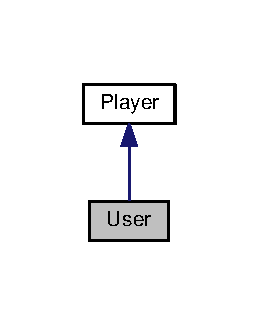
\includegraphics[width=124pt]{classUser__inherit__graph}
\end{center}
\end{figure}


Collaboration diagram for User\+:
\nopagebreak
\begin{figure}[H]
\begin{center}
\leavevmode
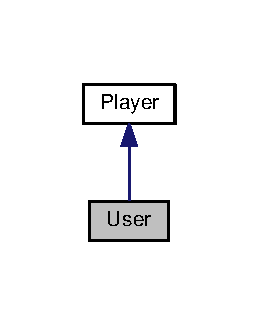
\includegraphics[width=124pt]{classUser__coll__graph}
\end{center}
\end{figure}
\subsection*{Public Member Functions}
\begin{DoxyCompactItemize}
\item 
\hyperlink{classUser_a7f5bdedd380237069e06d050569b9af1}{User} (\hyperlink{classGame}{Game} game, int id, int user\+Interface)
\begin{DoxyCompactList}\small\item\em Constructor. \end{DoxyCompactList}\item 
void \hyperlink{classUser_a29bbf7266caac4aae7aa26acf1f19592}{build\+Ships} ()  throws I\+O\+Exception 
\begin{DoxyCompactList}\small\item\em Build ships. \end{DoxyCompactList}\item 
void \hyperlink{classUser_a55aa9603904b16a22b91a357a32333ff}{attack} ()  throws I\+O\+Exception \hypertarget{classUser_a55aa9603904b16a22b91a357a32333ff}{}\label{classUser_a55aa9603904b16a22b91a357a32333ff}

\begin{DoxyCompactList}\small\item\em Attack the opponent\textquotesingle{}s \hyperlink{classShip}{Ship}\textquotesingle{}s. \end{DoxyCompactList}\end{DoxyCompactItemize}


\subsection{Detailed Description}
\hyperlink{classUser}{User} class. 

Class representing a user that plays a game. 

\subsection{Constructor \& Destructor Documentation}
\index{User@{User}!User@{User}}
\index{User@{User}!User@{User}}
\subsubsection[{\texorpdfstring{User(\+Game game, int id, int user\+Interface)}{User(Game game, int id, int userInterface)}}]{\setlength{\rightskip}{0pt plus 5cm}User.\+User (
\begin{DoxyParamCaption}
\item[{{\bf Game}}]{game, }
\item[{int}]{id, }
\item[{int}]{user\+Interface}
\end{DoxyParamCaption}
)\hspace{0.3cm}{\ttfamily [inline]}}\hypertarget{classUser_a7f5bdedd380237069e06d050569b9af1}{}\label{classUser_a7f5bdedd380237069e06d050569b9af1}


Constructor. 


\begin{DoxyParams}{Parameters}
{\em game} & \hyperlink{classGame}{Game} object. \\
\hline
{\em id} & id of a player. \\
\hline
\end{DoxyParams}


\subsection{Member Function Documentation}
\index{User@{User}!build\+Ships@{build\+Ships}}
\index{build\+Ships@{build\+Ships}!User@{User}}
\subsubsection[{\texorpdfstring{build\+Ships()}{buildShips()}}]{\setlength{\rightskip}{0pt plus 5cm}void User.\+build\+Ships (
\begin{DoxyParamCaption}
{}
\end{DoxyParamCaption}
) throws I\+O\+Exception\hspace{0.3cm}{\ttfamily [inline]}}\hypertarget{classUser_a29bbf7266caac4aae7aa26acf1f19592}{}\label{classUser_a29bbf7266caac4aae7aa26acf1f19592}


Build ships. 

A method to build ships. 

The documentation for this class was generated from the following file\+:\begin{DoxyCompactItemize}
\item 
src/User.\+java\end{DoxyCompactItemize}

%--- End generated contents ---

% Index
\backmatter
\newpage
\phantomsection
\clearemptydoublepage
\addcontentsline{toc}{chapter}{Index}
\printindex

\end{document}
